% SPI integrationstest

%tekst

I det følgende testes SPI kommunikationen. Alle kommandoer testes for sig og dokumenteres herunder ved logik analyse billeder samt tabeller der er udarbejdet af eksporterede .txt filer fra Salae Logic \footnote{Salae Logic er softwaren der benyttes til USB logic analyser. Det er herfra at analyse billeder samt data til tabellerne er fra}. 


% Aktiver
\textbf{Aktiver}

Aktiver kommandoen testes vha. testprogrammet ved kommandoen: 


\begin{figure}[H]
\centering
{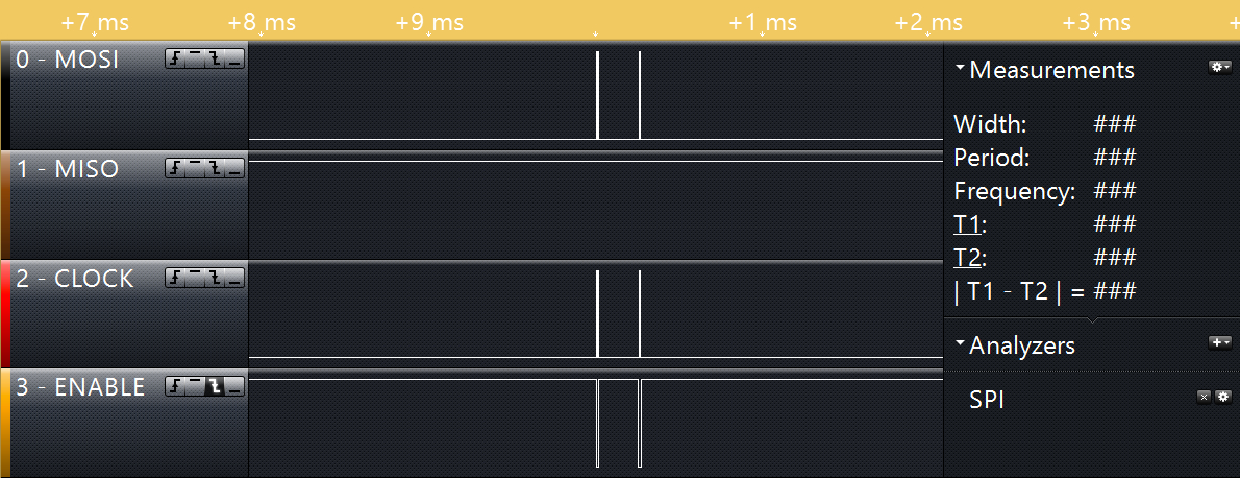
\includegraphics[width=0.90\textwidth]{filer/integrationstest/billeder/spi_activate}}
\caption{Analyse billede for kommandoen aktiver}
\label{lab:scop_activate}
\end{figure}

Tabel \ref{table:scop_activate} viser dataoverførelsen. Som det ses har kun MOSI betydning for aktiver, da aktiver er en write metode. 

\begin{table}[H]
	\caption{Analyse data eksporteret til tabel}
	\centering
	\begin{tabular}{|l|c|c|}
		\hline 
		\textbf{Char nr} & \textbf{0} & \textbf{1} \\ 		
		\hline 
		\textbf{MOSI} & '\verb+A+' & '\verb+C+' \\ 
		\hline 
		\textbf{MISO} & '\verb+255+' & '\verb+255+' \\ 
		\hline 
	\end{tabular} 
	\label{table:scop_activate}
\end{table}


% Deaktiver
\textbf{Deaktiver}
Deaktiver kommandoen testes vha. testprogrammet ved kommandoen: 


\begin{figure}[H]
\centering
{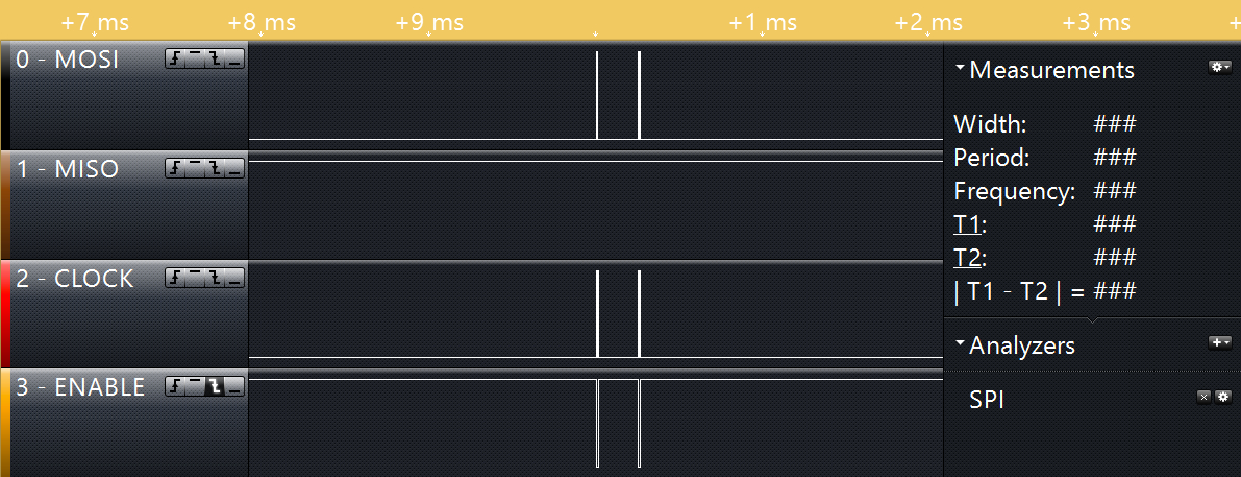
\includegraphics[width=0.90\textwidth]{filer/integrationstest/billeder/spi_deactivate}}
\caption{Analyse billede for kommandoen deaktiver}
\label{lab:scop_deactivate}
\end{figure}

Tabel \ref{table:scop_deactivate} viser dataoverførelsen. Som det ses har kun MOSI betydning for deaktiver, da deaktiver er en write metode. 

\begin{table}[h]
	\caption{Analyse data eksporteret til tabel}
	\centering
	\begin{tabular}{|l|c|c|}
		\hline 
		\textbf{Char nr} & \textbf{0} & \textbf{1} \\ 		
		\hline 
		\textbf{MOSI} & '\verb+D+' & '\verb+C+' \\ 
		\hline 
		\textbf{MISO} & '\verb+255+' & '\verb+255+' \\ 
		\hline 
	\end{tabular} 
	\label{table:scop_deactivate}
\end{table}


% Config
\textbf{Config}
Config kommandoen testes vha. testprogrammet ved kommandoen: 


\begin{figure}[H]
\centering
{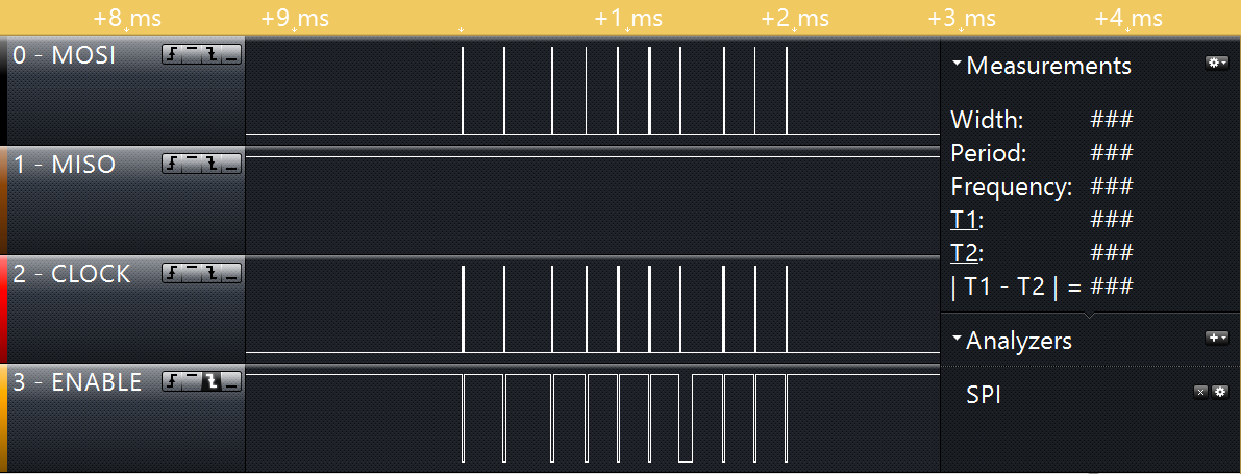
\includegraphics[width=0.90\textwidth]{filer/integrationstest/billeder/spi_config}}
\caption{Analyse billede for kommandoen config}
\label{lab:scop_config}
\end{figure}

Tabel \ref{table:scop_config} viser dataoverførelsen. Som det ses har kun MOSI betydning for config, da config er en write metode. 

\begin{table}[H]
	\caption{Analyse data eksporteret til tabel}
	\centering
	\begin{tabular}{|l|c|c|c|c|c|c|c|c|c|c|}
		\hline 
		\textbf{Char nr} & \textbf{0} & \textbf{1} & \textbf{2} & \textbf{3} & \textbf{4} & \textbf{5} 
						 & \textbf{6} & \textbf{7} & \textbf{8} & \textbf{9}\\ 		
		\hline 
		\textbf{MOSI} & '\verb+P+' & '\verb+1+' & '\verb+0+' & '\verb+0+' & '\verb+.+' & '\verb+1+' 
						& '\verb+0+' & '\verb+4+' & '\verb+8+' & '\verb+C+' \\ 
		\hline 
		\textbf{MISO} & '\verb+255+' & '\verb+255+' & '\verb+255+' & '\verb+255+' & '\verb+255+' & '\verb+255+' 
						& '\verb+255+' & '\verb+255+' & '\verb+255+' & '\verb+255+' \\ 
		\hline 
	\end{tabular} 
	\label{table:scop_config}
\end{table}


% Verificer
\textbf{Verificer}
Verificer kommandoen testes vha. testprogrammet ved kommandoen: 


\begin{figure}[H]
\centering
{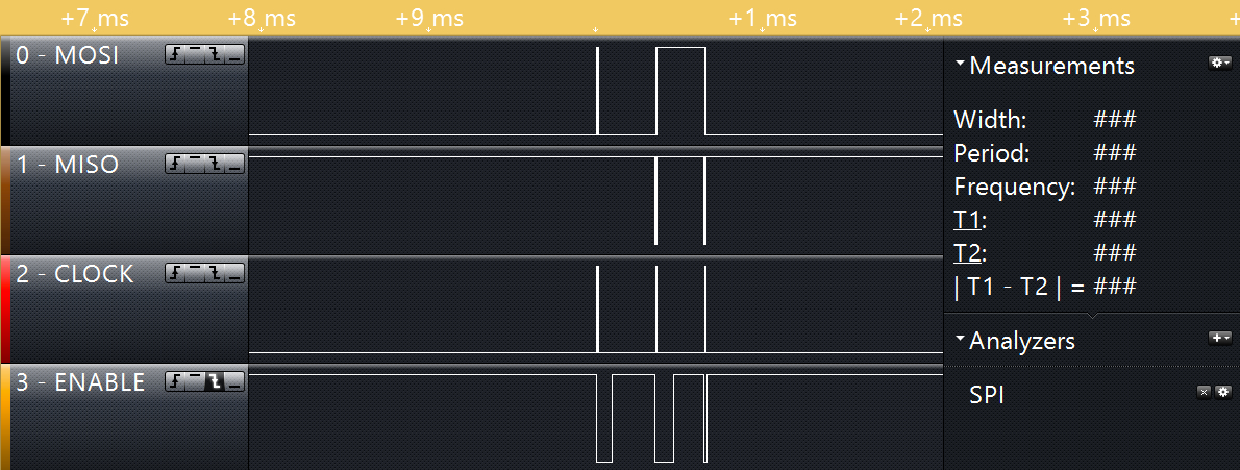
\includegraphics[width=0.90\textwidth]{filer/integrationstest/billeder/spi_verify}}
\caption{Analyse billede for kommandoen verificer}
\label{lab:scop_verify}
\end{figure}

Tabel \ref{table:scop_verify} viser dataoverførelsen. Som det ses overføres der data på både MOSI og MISO linjen. Det sker da verificer er en read-metode. Testen her er udført med tilkoblet Enhed. Hvis enheden kobles fra og der ikke modtages et matchende enhedsnummer, returneres en fejlkode i programmet. 
 

\begin{table}[H]
	\caption{Analyse data eksporteret til tabel}
	\centering
	\begin{tabular}{|l|c|c|c|}
		\hline 
		\textbf{Char nr} & \textbf{0} & \textbf{1} & \textbf{2}\\ 		
		\hline 
		\textbf{MOSI} & '\verb+V+' & '\verb+R+'  & '\verb+C+'\\ 
		\hline 
		\textbf{MISO} & '\verb+255+' & '\verb+1+' & '\verb+0+' \\ 
		\hline 
	\end{tabular} 
	\label{table:scop_verify}
\end{table}


% Log

\textbf{Log}
Getlog kommandoen testes vha. testprogrammet og med en test buffer i form af et char array "DTTT.TFFFVBEXXX" på Enheden: 

\begin{figure}[H]
\centering
{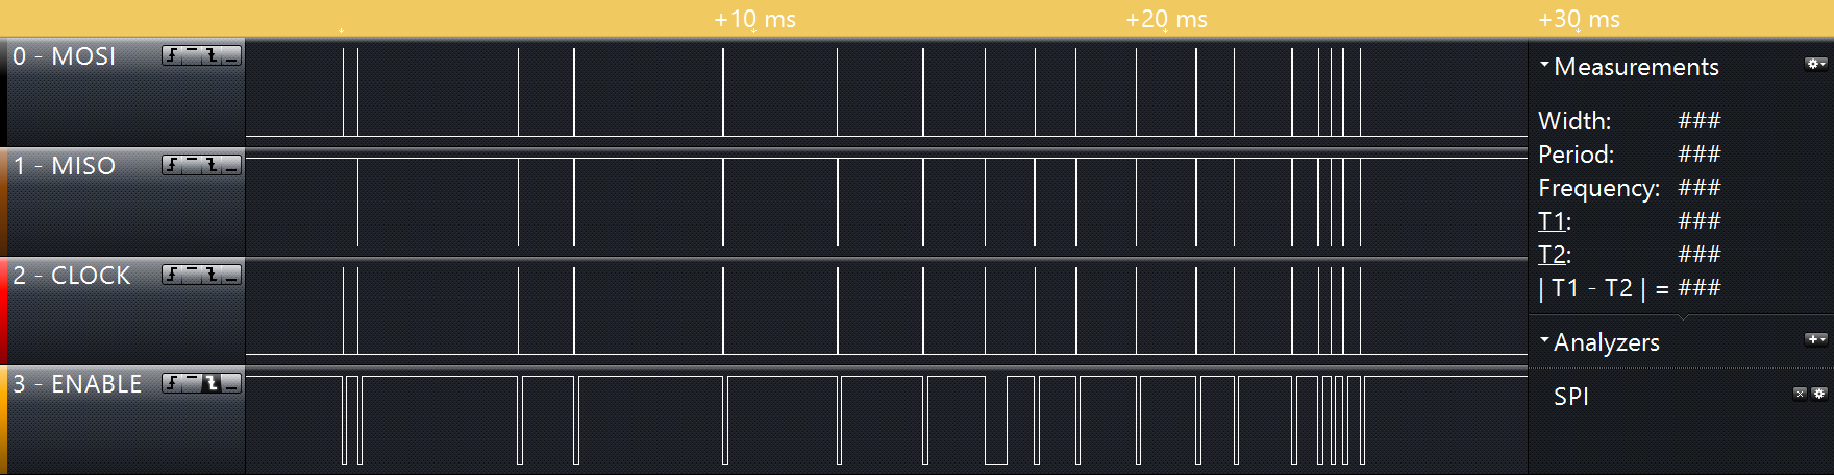
\includegraphics[width=0.90\textwidth]{filer/integrationstest/billeder/spi_getlog_and_error}}
\caption{Analyse billede for kommandoen getLog}
\label{lab:scop_getlog}
\end{figure}

Tabel \ref{table:scop_getlog1} og \ref{table:scop_getlog2} viser dataoverførelsen. 

\begin{table}[H]
	\caption{Analyse data eksporteret til tabel del 1}
	\centering
	\begin{tabular}{|l|c|c|c|c|c|c|c|c|c|c|}
		\hline 
		\textbf{Char nr} & \textbf{0} & \textbf{1} & \textbf{2} & \textbf{3} & \textbf{4} & \textbf{5} 
						 & \textbf{6} & \textbf{7} & \textbf{8} & \textbf{9}\\ 		
		\hline 
		\textbf{MOSI} & '\verb+L+' & '\verb+R+' & '\verb+R+' & '\verb+R+' & '\verb+R+' & '\verb+R+' 
						& '\verb+R+' & '\verb+R+' & '\verb+R+' & '\verb+R+'\\ 
		\hline 
		\textbf{MISO} & '\verb+255+' & '\verb+16+' & '\verb+D+' & '\verb+T+' & '\verb+T+' & '\verb+T+' 
						& '\verb+.+' & '\verb+T+' & '\verb+F+' & '\verb+F+'\\
						 
		\hline 
	\end{tabular} 
	\label{table:scop_getlog1}
\end{table}


\begin{table}[H]
	\caption{Analyse data eksporteret til tabel del 2}
	\centering
	\begin{tabular}{|l|c|c|c|c|c|c|c|c|}
		\hline 
		\textbf{Char nr} & \textbf{10} & \textbf{11} & \textbf{12} & \textbf{13}
						& \textbf{14} & \textbf{15} & \textbf{16} & \textbf{17}\\ 		
		\hline 
		\textbf{MOSI} 	& '\verb+R+' & '\verb+R+' & '\verb+R+' & '\verb+R+'
						& '\verb+R+' & '\verb+R+' & '\verb+R+' & '\verb+R+' \\ 
		\hline 
		\textbf{MISO}	& '\verb+F+' & '\verb+V+' & '\verb+B+' & '\verb+E+'
						& '\verb+X+' & '\verb+X+' & '\verb+X+' & '\verb+0+'\\
						 
		\hline 
	\end{tabular} 
	\label{table:scop_getlog2}
\end{table}

Der er ligeledes testet med et mere komplekst char array med flere data og error strenge. Disse læses også som de skal. 

\subsubsection*{Begrænsninger}

Ovenstående modultest er udført med et 7cm langt fladkabel til forbindelsen mellem Master og Enhed. Der er testet med et 22cm langt fladkabel, her var der en fejlrate på mere end 10\%. Ydermere er det nødvendigt at være opmærksom på ikke at lade nogle kabler krydse fladkablet, da dette giver støj og vil medføre fejl. Der er ikke oplevet fejl ved at benytte fladkablet på 7cm, så længe støjkilder holdes på afstand.   